\let\negmedspace\undefined
\let\negthickspace\undefined
\documentclass[journal,12pt,onecolumn]{IEEEtran}
\usepackage{cite}
\usepackage{amsmath,amssymb,amsfonts,amsthm}
\usepackage{algorithmic}
\usepackage{graphicx}
\graphicspath{{./figs/}}
\usepackage{textcomp}
\usepackage{xcolor}
\usepackage{txfonts}
\usepackage{listings}
\usepackage{enumitem}
\usepackage{mathtools}
\usepackage{gensymb}
\usepackage{comment}
\usepackage{caption}
\usepackage[breaklinks=true]{hyperref}
\usepackage{tkz-euclide} 
\usepackage{listings}
\usepackage{gvv}                                        
%\def\inputGnumericTable{}                                 
%\usepackage[latin1]{inputenc}     
\usepackage{xparse}
\usepackage{color}                                            
\usepackage{array}                                            
\usepackage{longtable}                                       
\usepackage{calc}                                             
\usepackage{multirow}
\usepackage{multicol}
\usepackage{hhline}                                           
\usepackage{ifthen}                                           
\usepackage{lscape}
\usepackage{tabularx}
\usepackage{array}
\usepackage{float}
\newtheorem{theorem}{Theorem}[section]
\newtheorem{problem}{Problem}
\newtheorem{proposition}{Proposition}[section]
\newtheorem{lemma}{Lemma}[section]
\newtheorem{corollary}[theorem]{Corollary}
\newtheorem{example}{Example}[section]
\newtheorem{definition}[problem]{Definition}
\newcommand{\BEQA}{\begin{eqnarray}}
\newcommand{\EEQA}{\end{eqnarray}}
\newcommand{\define}{\stackrel{\triangle}{=}}
\theoremstyle{remark}
\newtheorem{rem}{Remark}

\setlength{\tabcolsep}{15pt}
\renewcommand{\arraystretch}{1.75}

\begin{document}

\title{GATE 2023-CE}
\author{Pratyush Panda(AI25BTECH11024)}
\maketitle

\renewcommand{\thefigure}{\theenumi}
\renewcommand{\thetable}{\theenumi}

\section*{General Aptitude(GA)}
\section*{Q.1 - Q.5 Carry ONE mark Each}

\begin{enumerate}
\item “I have not yet decided what I will do this evening;I \underline{\hspace{2cm}} visit a friend.”

\hfill{\brak{\text{GATE CE-1 2023}}}
\begin{enumerate}
\item mite
\item would
\item might
\item didn't
\end{enumerate}

\item Eject : Insert : : Advance : \underline{\hspace{2cm}}
(By word meaning)

\hfill{\brak{\text{GATE CE-1 2023}}}
\begin{enumerate}
\item Advent
\item Progress
\item Retreat
\item Loan
\end{enumerate}

\item In the given figure, PQRSTV is a regular hexagon with each side of length $5 cm$. A
circle is drawn with its centre at V such that it passes through P. What is the area in \brak{\textit{$cm^2$}} of the shaded region? (The diagram is representative)

\hfill{\brak{\text{GATE CE-1 2023}}}
\begin{figure}[H]
\centering
\includegraphics[width = 0.5\columnwidth]{figs/q3.png}
\caption*{}
\label{fig:Q.3}
\end{figure}

\begin{enumerate}
\item \Large$\frac{25\pi}{3}$
\item \Large$\frac{20\pi}{3}$
\item \Large$6\pi$
\item \Large$7\pi$
\end{enumerate}

\item A duck named Donald Duck says “All ducks always lie.”
Based only on the information above, which one of the following statements can be logically inferred with certainty?

\hfill{\brak{\text{GATE CE-1 2023}}}
\begin{enumerate}
\item Donald Duck always lies.
\item Donald Duck always tells the truth.
\item Donald Duck’s statement is true.
\item Donald Duck’s statement is false. 
\end{enumerate}

\item A line of symmetry is defined as a line that divides a figure into two parts in a way such that each part is a mirror image of the other part about that line. The figure below consists of 20 unit squares arranged as shown. In addition to the given black squares, upto 5 more may be coloured black. Which one among the following options depicts the minimum number of boxes that must be coloured
black to achieve two lines of symmetry? (The figure is representative)

\hfill{\brak{\text{GATE CE-1 2023}}}
\begin{figure}[H]
\centering
\includegraphics[width=0.5\linewidth]{figs/q5.png}
\caption*{}
\label{fig:Q.5}
\end{figure}

\begin{enumerate}
\item d
\item c,d,i
\item c,i
\item c,d,i,f,g
\end{enumerate}

\section*{Q.6 – Q.10 Carry TWO marks Each}

\item Based only on the truth of the statement ‘Some humans are intelligent’, which one of the following options can be logically inferred with certainty?

\hfill{\brak{\text{GATE CE-1 2023}}}
\begin{enumerate}
\item No human is intelligent.
\item All humans are intelligent. 
\item Some non-humans are intelligent.
\item Some intelligent beings are humans.
\end{enumerate}

\item Which one of the options can be inferred about the mean, median, and mode for the given probability distribution (i.e. probability mass function), $P(x)$, of a variable x?

\hfill{\brak{\text{GATE CE-1 2023}}}
\begin{figure}[H]
\centering
\includegraphics[width=0.5\linewidth]{figs/q7.png}
\caption*{}
\label{fig:Q.7}
\end{figure}

\begin{enumerate}
\item $mean = median \neq mode$
\item $mean = median = mode$
\item $mean \neq median = mode$
\item $mean \neq mode = median$
\end{enumerate}

\item The James Webb telescope, recently launched in space, is giving humankind unprecedented access to the depths of time by imaging very old stars formed almost 13 billion years ago. Astrophysicists and cosmologists believe that this odyssey in space may even shed light on the existence of dark matter. Dark matter is supposed to interact only via the gravitational interaction and not through the electromagnetic-, the weak- or the strong-interaction. This may justify the epithet “dark” in dark matter.\\
Based on the above paragraph, which one of the following statements is FALSE?

\hfill{\brak{\text{GATE CE-1 2023}}}
\begin{enumerate}
\item No other telescope has captured images of stars older than those captured by the James Webb telescope.
\item People other than astrophysicists and cosmologists may also believe in the existence of dark matter.
\item The James Webb telescope could be of use in the research on dark matter.
\item If dark matter was known to interact via the strong-interaction, then the epithet “dark” would be justified.
\end{enumerate}

\item Let $a = 30!$ , $b = 50!$ , and $c = 100!$ . Consider the following numbers:\\
$\log_{a}c$,\hspace{2cm} $\log_{c}a$,\hspace{2cm} $\log_{b}a$, \hspace{2cm} $\log_{a}b$\\
Which one of the following inequalities is CORRECT?

\hfill{\brak{\text{GATE CE-1 2023}}}
\begin{enumerate}
\item $\log_{c}a$ < $\log_{b}a$ < $\log_{a}b$ < $\log_{a}c$
\item $\log_{c}a$ < $\log_{a}b$ < $\log_{b}a$ < $\log_{b}c$
\item $\log_{c}a$ < $\log_{b}a$ < $\log_{a}c$ < $\log_{a}b$
\item $\log_{b}a$ < $\log_{c}a$ < $\log_{a}b$ < $\log_{a}c$
\end{enumerate}

\item A square of side length 4 cm is given. The boundary of the shaded region is defined by one semi-circle on the top and two circular arcs at the bottom, each of radius $2 cm$, as shown.\\
The area of the shaded region is \underline{\hspace{2cm}}$cm^2$

\hfill{\brak{\text{GATE CE-1 2023}}}
\begin{figure}[H]
\centering
\includegraphics[width = 0.5\columnwidth]{figs/q10.png}
\caption*{}
\label{fig:Q.10}
\end{figure}

\begin{enumerate}
\item 8
\item 4
\item 12
\item 10
\end{enumerate}

\section*{Q.11 – Q.35 Carry ONE mark Each}

\item for the integral \\
\begin{center}
\Large\textbf{$\int_{a}^{b} f(x) \,dx$}
\end{center}

which of the following statements is TRUE?

\hfill{\brak{\text{GATE CE-1 2023}}}
\begin{enumerate}
\item I=0
\item I=2
\item I=-2
\item the integral does not converge.
\end{enumerate}

\item A hanger is made of two bars of different sizes. Each bar has a square cross-section. The hanger is loaded by three-point loads in the mid vertical plane as shown in the figure. Ignore the self-weight of the hanger. What is the maximum tensile stress in $N/mm^2$ anywhere in the hanger without considering stress concentration effects?

\hfill{\brak{\text{GATE CE-1 2023}}}
\begin{figure}[H]
\centering
\includegraphics[width=0.5\linewidth]{figs/q12.png}
\caption*{}
\label{fig:Q.12}
\end{figure}

\begin{enumerate}
\item 15.0
\item 25.0
\item 35.0
\item 45.0
\end{enumerate}

\item Creep of concrete under compression is defined as the \underline{\hspace{2cm}}.

\hfill{\brak{\text{GATE CE-1 2023}}}
\begin{enumerate}
\item increase in the magnitude of strain under constant stress.
\item increase in the magnitude of stress under constant strain
\item decrease in the magnitude of strain under constant stress
\item decrease in the magnitude of stress under constant strain
\end{enumerate}

\item A singly reinforced concrete beam of balanced section is made of M20 grade concrete and Fe415 grade steel bars. The magnitudes of the maximum compressive strain in concrete and the tensile strain in the bars at ultimate state under flexure, as per IS $456: 2000$ are \underline{\hspace{2cm}}, respectively.(\textit{round off to four decimal places})

\hfill{\brak{\text{GATE CE-1 2023}}}
\begin{enumerate}
\item 0.0035 and 0.0038
\item 0.0020 and 0.0018
\item 0.0035 and 0.0041
\item 0.0020 and 0.0031
\end{enumerate}

\item In cement concrete mix design, with the increase in water-cement ratio, which one of the following statements is TRUE?

\hfill{\brak{\text{GATE CE-1 2023}}}
\begin{enumerate}
\item Compressive strength decreases but workability increases
\item Compressive strength increases but workability decreases
\item Both compressive strength and workability decrease
\item Both compressive strength and workability increase
\end{enumerate}

\item The specific gravity of a soil is $2.60$. The soil is at $50\%$ degree of saturation with a water content of $15\%$. The void ratio of the soil is \underline{\hspace{2cm}}

\hfill{\brak{\text{GATE CE-1 2023}}}
\begin{enumerate}
\item $0.35$
\item $0.78$
\item $0.87$
\item $1.28$
\end{enumerate}

\item A group of 9 friction piles are arranged in a square grid maintaining equal spacing in all directions. Each pile is of diameter $300 mm$ and length $7 m$. Assume that the soil is cohesionless with effective friction angle $\phi$ = 32°. What is the center-to-center spacing of the piles (in $m$) for the pile group efficiency of $60\%$?

\hfill{\brak{\text{GATE CE-1 2023}}}
\begin{enumerate}
\item $0.582$
\item $0.486$
\item $0.391$
\item $0.677$
\end{enumerate}

\item A possible slope failure is shown in the figure. Three soil samples are taken from different locations (I, II and III) of the potential failure plane. Which is the most appropriate shear strength test for each of the sample to identify the failure mechanism? Identify the correct combination from the following options:

\hfill{\brak{\text{GATE CE-1 2023}}}
\begin{itemize}
\item P: Triaxial compression test
\item Q: Triaxial extension test
\item R: Direct shear or shear box test
\item S: Vane shear test
\end{itemize}

\begin{figure}[H]
\centering
\includegraphics[width=0.5\linewidth]{figs/q18.png}
\caption*{}
\label{fig:Q.18}
\end{figure}

\begin{enumerate}
\item I-Q, II-R, III-P
\item I-R, II-P, III-Q
\item I-S, II-Q, III-R
\item I-P, II-R, III-Q
\end{enumerate}

\item When a supercritical stream enters a mild-sloped (M) channel section, the type of flow profile would become \underline{\hspace{2cm}}.

\hfill{\brak{\text{GATE CE-1 2023}}}
\begin{enumerate}
\item $M_1$
\item $M_2$
\item $M_3$
\item $M_1$ and $M_2$
\end{enumerate}

\item Which one of the following statements is TRUE for Greenhouse Gas (GHG) in the atmosphere?

\hfill{\brak{\text{GATE CE-1 2023}}}
\begin{enumerate}
\item GHG absorbs the incoming short wavelength solar radiation to the earth surface and allows the long wavelength radiation coming from the earth surface to pass through
\item GHG allows the incoming long wavelength solar radiation to pass through to the earth surface, and absorbs the short wavelength radiation coming from the earth surface
\item GHG allows the incoming long wavelength solar radiation to pass through to the earth surface, and allows the short wavelength radiation coming from the earth surface to pass through
\item GHG allows the incoming short wavelength solar radiation to pass through to the earth surface, and absorbs the long wavelength radiation coming from the earth surface
\end{enumerate}

\item $G_1$ and $G_2$ are the slopes of the approach and departure grades of a vertical curve, respectively.

Given $|G_1| < |G_2|$ and $|G_1| \neq |G_2| \neq 0$\\
Statement 1: $+G_1$ followed by $+G_2$ results in a sag vertical curve.\\
Statement 2: $-G_1$ followed by $-G_2$ results in a sag vertical curve.\\
Statement 3: $+G_1$ followed by $-G_2$ results in a crest vertical curve.\\

Which option amongst the following is true?

\hfill{\brak{\text{GATE CE-1 2023}}}
\begin{enumerate}
\item Statement 1 and Statement 3 are correct; Statement 2 is wrong
\item Statement 1 and Statement 2 are correct; Statement 3 is wrong
\item Statement 1 is correct; Statement 2 and Statement 3 are wrong
\item Statement 2 is correct; Statement 1 and Statement 3 are wrong
\end{enumerate}

\item The direct and reversed zenith angles observed by a theodolite are $56^\circ 00' 00''$ and $303^\circ 00' 00''$, respectively. What is the vertical collimation correction?

\hfill{\brak{\text{GATE CE-1 2023}}}
\begin{enumerate}
\item $+1^\circ 00' 00''$
\item $-1^\circ 00' 00''$
\item $-0^\circ 30' 00''$
\item $+0^\circ 30' 00''$
\end{enumerate}

\item A student is scanning his $10 inch\times10 inch$ certificate at $600$ dots per inch (dpi) to convert it to raster. What is the percentage reduction in number of pixels if the same certificate is scanned at $300$ dpi?

\hfill{\brak{\text{GATE CE-1 2023}}}
\begin{enumerate}
\item $62$
\item $88$
\item $75$
\item $50$
\end{enumerate}

\item If M is an arbitrary real n × n matrix, then which of the following matrices will have non-negative eigenvalues?

\hfill{\brak{\text{GATE CE-1 2023}}}
\begin{enumerate}
\item $M^2$
\item M$M^T$
\item $M^T$M
\item $(M^T)^2$
\end{enumerate}

\item The following function is defined over the interval $[-L, L]$:\\
$f(x) = px^4 + qx^5.$

If it is expressed as a Fourier series,\\
$f(x) = a_0 + \sum_{n=1}^{\infty} \left\{ a_n \sin\left(\frac{n\pi x}{L}\right) + b_n \cos\left(\frac{n\pi x}{L}\right) \right\}$\\
which options amongst the following are true?

\hfill{\brak{\text{GATE CE-1 2023}}}
\begin{enumerate}
\item $a_n, n=1,2,\cdots,\infty$ depend on $p$
\item $a_n, n=1,2,\cdots,\infty$ depend on $q$
\item $b_n, n=1,2,\cdots,\infty$ depend on $p$
\item $b_n, n=1,2,\cdots,\infty$ depend on $q$
\end{enumerate}

\item Consider the following three structures

\begin{figure}[H]
\centering
\includegraphics[width=0.5\linewidth]{figs/q26.png}
\caption*{}
\label{fig:Q.26}
\end{figure}

Which of the folloing statements is/are TRUE?

\hfill{\brak{\text{GATE CE-1 2023}}}
\begin{enumerate}
\item Structure I is unstable.
\item Structure II is unstable
\item Structure III is unstable
\item All three structures are stable
\end{enumerate}

\item Identify the waterborne diseases caused by viral pathogens:

\hfill{\brak{\text{GATE CE-1 2023}}}
\begin{enumerate}
\item Acute anterior poliomyelitis
\item Cholera
\item Infectious hepatitis
\item Typhoid fever
\end{enumerate}

\item Which of the following statements is/are TRUE for the Refuse-Derived Fuel (RDF) in the context of Municipal Solid Waste (MSW) management?

\hfill{\brak{\text{GATE CE-1 2023}}}
\begin{enumerate}
\item Higher Heating Value (HHV) of the unprocessed MSW is higher than the HHV of RDF processed from the same MSW
\item RDF can be made in the powdered form
\item Inorganic fraction of MSW is mostly converted to RDF
\item RDF cannot be used in conjunction with oil
\end{enumerate}

\item The probabilities of occurrences of two independent events A and B are $0.5$ and $0.8$, respectively. What is the probability of occurrence of at least A or B (rounded off to one decimal place) \underline{\hspace{3cm}}

\hfill{\brak{\text{GATE CE-1 2023}}}

\item In the diffrential equation $\frac{dy}{dx}+\alpha xy=0$, $\alpha$ is a positive constant. If $y=1.0$ at $x=0.0$ and $y=0.8$ at $x=1.0$, the value of $\alpha$ is \underline{\hspace{2cm}} $\brak{\textit{round off to the nearest integer}}$

\hfill{\brak{\text{GATE CE-1 2023}}}

\item Consider the fillet-welded lap joint shown in the figure $\brak{not to scale}$. The length of the weld shown is the effective length. The welded surfaces meet at right angle. The weld size is $8 mm$, and the permissible stress in the weld is $120MPa$. What is the safe load P $\brak{in kN, rounded off to one decimal place}$ that can be transmitted by this welded joint? \underline{\hspace{2cm}}

\hfill{\brak{\text{GATE CE-1 2023}}}

\begin{figure}[H]
\centering
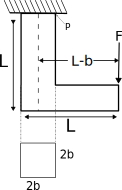
\includegraphics[width=0.5\linewidth]{figs/q31.png}
\caption*{}
\label{fig:Q.31}
\end{figure}

\item A drained direct shear test was carried out on a sandy soil. Under a normal stress of $50kPa$, the test specimen failed at a shear stress of $35kPa$. The angle of internal friction of the sample is \underline{\hspace{2cm}} degrees $\brak{\textit{round off to the nearest integer}}$

\hfill{\brak{\text{GATE CE-1 2023}}}

\item A canal supplies water to an area growing wheat over $100$ hectares. The duration between the first and last watering is $120$ days, and the total depth of water required by the crop is $35 cm$. The most intense watering is required over a period of $30$ days and requires a total depth of water equal to $12 cm$. Assuming precipitation to be negligible and neglecting all losses, the minimum discharge (in $m^3/s$, rounded off to three decimal places) in the canal to satisfy the crop requirement is \underline{\hspace{3cm}}

\hfill{\brak{\text{GATE CE-1 2023}}}

\item The ordinates of a one-hour unit hydrograph for a catchment are given below:
\begin{table}[H]
\centering
\begin{tabular}{|c|c|c|c|c|c|c|c|c|}
\hline
t (hour) & 0 & 1 & 2 & 3 & 4 & 5 & 6 & 7\\
\hline
Q ($m^3/s$) & 0 & 9 & 21 & 18 & 12 & 5 & 2 & 0\\
\hline
\end{tabular}
\end{table}
Using the principle of superposition, a D-hour unit hydrograph for the catchment was derived from this one-hour unit hydrograph. The ordinates of the D-hour unit hydrograph were obtained as $3 m^3/s$ at $t = 1 hour$ and 10 $m^3/s$ at $t = 2 hour$. The value of D $\brak{\textit{in integer}}$ is \underline{\hspace{3cm}}

\hfill{\brak{\text{GATE CE-1 2023}}}

\item For a horizontal curve, the radius of a circular curve is obtained as $300 m$ with the design speed as $15 m/s$. If the allowable jerk is $0.75 m/s^3$ , what is the minimum length in m, $\brak{\textit{in integer}}$ of the transition curve? \underline{\hspace{3cm}}

\hfill{\brak{\text{GATE CE-1 2023}}}

\section*{Q.36 – Q.65 Carry TWO marks Each}

\item A function $f(x)$, that is smooth and convex-shaped between interval $\brak{x_l,x_u}$ is shown in the figure. This function is observed at odd number of regularly spaced points. If the area under the function is computed numerically, then \underline{\hspace{2cm}}

\hfill{\brak{\text{GATE CE-1 2023}}}
\begin{figure}[H]
\centering
\includegraphics[width=0.5\linewidth]{figs/q36.png}
\caption*{}
\label{fig:Q.36}
\end{figure}

\begin{enumerate}
\item the numerical value of the area obtained using the trapezoidal rule will be less than the actual
\item the numerical value of the area obtained using the trapezoidal rule will be more than the actual
\item the numerical value of the area obtained using the trapezoidal rule will be exactly equal to the actual
\item with the given details, the numerical value of area cannot be obtained using trapezoidal rule
\end{enumerate}

\item Consider a doubly reinforced RCC beam with the option of using either Fe250 plain bars or Fe500 deformed bars in the compression zone. The modulus of elasticity of steel is $2 \times 10^5 N/mm^2$. As per IS456:2000, in which type(s) of the bars, the stress in the compression steel $\brak{f_(fc)}$ can reach the design strength $\brak{0.87f_y}$ at the limit state of collapse?

\hfill{\brak{\text{GATE CE-1 2023}}}
\begin{enumerate}
\item Fe250 plain bars only
\item Fe250 plain bars only
\item Both Fe250 plain bars and Fe500 deformed bars
\item Neither Fe250 plain bars nor Fe500 deformed bars
\end{enumerate}

\item Consider the horizontal axis passing through the centroid of the steel beam crosssection shown in the figure. What is the shape factor (rounded off to one decimal place) for the cross-section?

\hfill{\brak{\text{GATE CE-1 2023}}}
\begin{figure}[H]
\centering
\includegraphics[width=0.5\linewidth]{figs/q38.png}
\caption*{}
\label{fig:Q.38}
\end{figure}
\begin{enumerate}
\item $1.5$
\item $1.7$
\item $1.3$
\item $2.0$
\end{enumerate}

\item Consider the pin-jointed truss shown in the figure (not to scale). All members have the same axial rigidity, $AE$. Members $QR$
$RS$ and $ST$ have the same length $L$. Angles $QBT$, $RCT$, $SDT$ are all $90^\circ$. Angles $BQT$, $CRT$, $DST$ are all $30^\circ$. The joint $T$ carries a vertical load $P$. The vertical deflection of joint $T$ is $k\frac{PL}{AE}$. What is the value of $k$?

\hfill{\brak{\text{GATE CE-1 2023}}}
\begin{figure}[H]
\centering
\includegraphics[width=0.5\linewidth]{figs/q39.png}
\caption*{}
\label{fig:Q.39}
\end{figure}
\begin{enumerate}
\item $1.5$
\item $4.5$
\item $3.0$
\item $9.0$
\end{enumerate}

\item With reference to the compaction test conducted on soils, which of the following is INCORRECT?

\hfill{\brak{\text{GATE CE-1 2023}}}
\begin{enumerate}
\item Peak point of the compaction curve gives the maximum dry unit weight and optimum moisture content
\item With increase in the compaction effort, the maximum dry unit weight increases
\item With increase in the compaction effort, the optimum moisture content decreases
\item Compaction curve crosses the zero-air-voids curve
\end{enumerate}

\item Consider that a force $P$ is acting on the surface of a half-space (Boussinesq’s problem). The expression for vertical stress $\brak{\sigma_z}$ at any point $\brak{r,z}$, within the half-space is given as,

\begin{center}
\Large$\sigma_z=\frac{3P}{2\pi}\frac{z^3}{\brak{r^2+z^2}^\frac{5}{2}}$
\end{center}

where, $r$ is the radial distance, and $z$ is the depth with downward direction taken as positive. At any given $r$, there is a variation of $\sigma_z$ along $z$ axis, and at a specific $z$, the value of $\sigma_z$ will be maximum. What is the locus of the maximum $\sigma_z$?

\hfill{\brak{\text{GATE CE-1 2023}}}
\begin{enumerate}
\item $z^2=\frac{3}{2}r^2$
\item $z^3=\frac{3}{2}r^2$
\item $z^2=\frac{5}{2}r^2$
\item $z^3=\frac{5}{2}r^2$
\end{enumerate}

\item A square footing of size $2.5m\times2.5m$ is placed $1.0m$ m below the ground surface on a cohesionless homogeneous soil stratum. Considering that the groundwater table is located at the base of the footing, the unit weights of soil above and below the groundwater table are $18kN/m^3$ and $20kN/m^3$, respectively, and the bearing capacity factor $N_q$ is 58, the net ultimate bearing capacity of the soil is estimated as $1706kPa$ $\brak{unit weight of water=10kN/m^3}$\\
Earlier, a plate load test was carried out with a circular plate of $30cm$ diameter in the same foundation pit during a dry season, when the water table was located beyond the plate influence zone. Using Terzaghi’s bearing capacity formulation, what is the ultimate bearing capacity $\brak{in kPa}$ of the plate?

\hfill{\brak{\text{GATE CE-1 2023}}}
\begin{enumerate}
\item $110.16$
\item $61.20$
\item $204.00$
\item $163.20$
\end{enumerate}

\item A very wide rectangular channel carries a discharge $\brak{Q}$ of $70 m^3/s$ per meter width. Its bed slope changes from $0.0001$ to $0.0009$ at a point P, as shown in the figure $\brak{\textit{not to scale}}$. The Manning’s roughness coefficient of the channel is $0.01$. What water surface profile(s) exist(s) near the point P?

\hfill{\brak{\text{GATE CE-1 2023}}}
\begin{figure}[H]
\centering
\includegraphics[width=0.5\linewidth]{figs/q43.png}
\caption{Caption}
\label{fig:Q.43}
\end{figure}
\begin{enumerate}
\item $M_2$ and $S_2$
\item $M_2$ only
\item $S_2$ only
\item $S_2$ and hydraulic jump
\end{enumerate}

\item A jet of water having a velocity of $20m/s$ strikes a series of plates fixed radially on a wheel revolving in the same direction as the jet at $15m/s$. What is the percentage efficiency of the plates? $\brak{\textit{round off to one decimal place}}$

\hfill{\brak{\text{GATE CE-1 2023}}}
\begin{enumerate}
\item $37.5$
\item $66.7$
\item $50.0$
\item $88.9$
\end{enumerate}

\item In the following table, identify the correct set of associations between the entries in Column-1 and Column-2.

\hfill{\brak{\text{GATE CE-1 2023}}}
\begin{table}[H]
\centering
\begin{tabular}{|l|l|}
\hline
Column-1 & Column-2 \\
\hline
P: Reverse Osmosis & $I$: Ponding \\
\hline
Q: Trickling Fliter & $II$: Freundlich Isotherm \\
\hline
R: Coagulation & $III$: Concentration Polarisation \\
\hline
S: Adsorbtion & $IV$: Charge Neutralisation\\
\hline
\end{tabular}
\end{table}
\begin{enumerate}
\item $P-II$, $Q-I$, $S-III$
\item $Q-III$, $R-II$, $S-IV$
\item $P-IV$, $R-I$, $S-II$
\item $P-III$, $Q-I$, $R-IV$
\end{enumerate}

\item A plot of speed-density relationship $\brak{\textit{linear}} $of two roads $\brak{\text{Road A and Road B}}$ is shown in the figure.
\begin{figure}[H]
\centering
\includegraphics[width=0.5\linewidth]{figs/q46.png}
\caption*{}
\label{fig:Q.46}
\end{figure}

If the capacity of Road A is $C_A$ and the capacity of Road B is $C_B$, what is $\frac{C_A}{C_B}$?

\hfill{\brak{\text{GATE CE-1 2023}}}
\begin{enumerate}
\item $\frac{k_A}{k_B}$
\item $\frac{u_A}{u_B}$
\item $\frac{k_Au_A}{k_Bu_B}$
\item $\frac{k_Au_B}{k_Bu_A}$
\end{enumerate}

\item For the matrix.
$\vec{A} = \myvec{1 & 2 & 3 \\
3 & 2 & 1 \\
3 & 1 & 2
}$
Which of the following statement is/are TRUE?

\hfill{\brak{\text{GATE CE-1 2023}}}
\begin{enumerate}
\item The eigenvalue of $\sbrak{A}^T$ are the same as eigenvalue of  $\sbrak{A}$
\item The eigenvalue of $\sbrak{A}^{-1}$ are the reciprocal of the eigenvalue of  $\sbrak{A}$
\item The eigenvectors of $\sbrak{A}^T$ are the same as eigenvectors of  $\sbrak{A}$
\item The eigenvectors of $\sbrak{A}^{-1}$ are the same as the eigenvectors of  $\sbrak{A}$
\end{enumerate}

\item For the function $f(x)=e^x|\sin{x}|$; $x\in\mathbb{R}$, which of the folloing statements is/are TRUE?

\hfill{\brak{\text{GATE CE-1 2023}}}
\begin{enumerate}
\item The function is continuous at all $x$
\item The function is differentiable at all $x$
\item The function is periodic
\item The function is bounded
\end{enumerate}

\item Consider the beam shown in the figure $\brak{\textit{not to scale}}$, on a hinge support at end A and a roller support at end B. The beam has a constant flexural rigidity, and is subjected to the external moments of magnitude $M$ at one-third spans, as shown in the figure. Which of the following statements is/are TRUE?

\hfill{\brak{\text{GATE CE-1 2023}}}
\begin{figure}[H]
\centering
\includegraphics[width=0.5\linewidth]{figs/q49.png}
\caption*{}
\label{fig:Q.49}
\end{figure}

\begin{enumerate}
\item Support reactions are zero
\item Shear force is zero everywhere
\item Bending moment is zero everywhere
\item Deflection is zero everywhere
\end{enumerate}

\item Which of the following statements is/are TRUE in relation to the Maximum Mixing Depth $\brak{\text{or Height}}$ ‘$D_{max}$’ in the atmosphere?

\hfill{\brak{\text{GATE CE-1 2023}}}
\begin{enumerate}
\item $D_{max}$ is always equal to the height of the layer of unstable air
\item Ventilation coefficient depends on $D_{max}$
\item A smaller $D_{max}$ will have a smaller air pollution potential if other meteorological conditions remain same
\item Vertical dispersion of pollutants occurs up to $D_{max}$
\end{enumerate}

\item Which of the following options match the test reporting conventions with the given material tests in the table?

\hfill{\brak{\text{GATE CE-1 2023}}}
\begin{table}[H]
\centering
\begin{tabular}{|l|l|}
\hline
\textbf{Test reporting convention} & \textbf{Material test}\\
\hline
(P) Reported as ratio & (I)Solubility of bitumen\\
\hline
(Q) Reported as percentage & (II) Softening points of bitumen\\
\hline
(R) Reported in temperature & (III) Los Angeles abrasion test\\
\hline
(S) Reported in length & (IV) Flash point of bitumen\\
\hline
 & (V) Ductility of bitumen\\
\hline
 & (VI) Specific gravity of bitumen\\
\hline
 & (VII) hin film oven test\\
\hline
\end{tabular}
\end{table}

\begin{enumerate}
\item (P) - (VI); (Q) - (I); (R) - (II); (S) - (VII)
\item (P) - (VI); (Q) - (III); (R) - (IV); (S) - (V)
\item (P) - (VI); (Q) - (I); (R) - (II); (S) - (V)
\item (P) - (VI); (Q) - (III); (R) - (IV); (S) - (VII)
\end{enumerate}

\item the differential equation,

\begin{center}
$\frac{du}{dt}+2tu^2=1$
\end{center}

is solved by employing a backward difference scheme within the finite difference framework. The value of $u$ at the $\brak{n-1}^{th}$ time-step, for some $n$ is 1.75. The corresponding time $\brak{\textit{t}}$ is $3.14s$. Each time-step is $0.01s$ long. Then the value of $\brak{u_n-u_{n-1}}$ is \underline{\hspace{3cm}} $\brak{\textit{round off to three decimal places}}$.

\hfill{\brak{\text{GATE CE-1 2023}}}

\item The infinitesimal element shown in the figure $\brak{\textit{not to scale}}$ represents the state of stress at a point in a body. What is the magnitude of the maximum principal stress $\brak{\text{in} N/mm^2, \textit{in integer}}$ at the point? \underline{\hspace{3cm}}

\hfill{\brak{\text{GATE CE-1 2023}}}
\begin{figure}[H]
\centering
\includegraphics[width=0.5\linewidth]{figs/q53.png}
\caption*{}
\label{fig:Q.53}
\end{figure}

\item An idealised bridge truss is shown in the figure. The force in member $U_2L_3$ is \underline{\hspace{3cm}}$kN$ $\brak{\textit{round off to one decimal place}}$

\hfill{\brak{\text{GATE CE-1 2023}}}
\begin{figure}[H]
\centering
\includegraphics[width=0.5\linewidth]{figs/q54.png}
\caption*{}
\label{fig:Q.54}
\end{figure}

\item The cross-section of a girder is shown in the figure $\brak{\text{not to scale}}$. The section is symmetric about a vertical axis $\brak{\text{Y-Y}}$. The moment of inertia of the section about the horizontal axis $\brak{\text{X-X}}$ passing through the centroid is \underline{\hspace{2cm}} $cm^4$ $\brak{\textit{round off to nearest integer}}$.

\hfill{\brak{\text{GATE CE-1 2023}}}
\begin{figure}[H]
\centering
\includegraphics[width=0.5\linewidth]{figs/q55.png}
\caption*{}
\label{fig:Q.55}
\end{figure}

\item A soil having the average properties, bulk unit weight = $19 kN/m^3$; angle of internal friction = $25^\circ$ and cohesion = $15 kPa$, is being formed on a rock slope existing at an inclination of $35^\circ$ with the horizontal. The critical height $\brak{\text{in m}}$ of the soil formation up to which it would be stable without any failure is \underline{\hspace{2cm}} $\brak{\textit{(round
off to one decimal place}}$.\\
$\sbrak{\text{Assume the soil is being formed parallel to the rock bedding plane and there is no
ground water effect.}}$

\hfill{\brak{\text{GATE CE-1 2023}}}

\item A smooth vertical retaining wall supporting layered soils is shown in figure. According to Rankine’s earth pressure theory, the lateral active earth pressure acting at the base of the wall is \underline{\hspace{2cm}}$kPa$ $\brak{\textit{(round
off to one decimal place}}$

\hfill{\brak{\text{GATE CE-1 2023}}}
\begin{figure}[H]
    \centering
    \includegraphics[width=0.5\linewidth]{figs/q57.png}
    \caption*{}
    \label{fig:Q.57}
\end{figure}

\item A vertical trench is excavated in a clayey soil deposit having a surcharge load of $30 kPa$. A fluid of unit weight $12 kN/m^3$
is poured in the trench to prevent collapse as the excavation proceeds. Assume that the fluid is not seeping through the soil
deposit. If the undrained cohesion of the clay deposit is $20 kPa$ and saturated unit weight is $18 kN/m^3$ , what is the maximum depth of unsupported excavation $\brak{\textit{in m,
rounded off to two decimal places}}$? \underline{\hspace{3cm}}

\hfill{\brak{\text{GATE CE-1 2023}}}

\item A 12-hour storm occurs over a catchment and results in a direct runoff depth of $100 mm$. The time-distribution of the rainfall intensity is shown in the figure $\brak{\text{not to scale}}$. The $\phi$-index of the storm is $\brak{\textit{in mm, rounded off to two decimal places}}$ \underline{\hspace{3cm}}

\hfill{\brak{\text{GATE CE-1 2023}}}
\begin{figure}[H]
    \centering
    \includegraphics[width=0.5\linewidth]{figs/q59.png}
    \caption*{}
    \label{fig:Q.59}
\end{figure}

\item A hydraulic jump occurs in a $1.0 m$ wide horizontal, frictionless, rectangular channel, with a pre-jump depth of $0.2 m$ and a post-jump depth of $1.0 m$. The value of g may be taken as $10 m/s^2$ . The values of the specific force at the pre-jump and post-jump sections are same and are equal to $\brak{\textit{in $m^3$
, rounded off to two decimal places}}$ \underline{\hspace{3cm}}.

\hfill{\brak{\text{GATE CE-1 2023}}}

\item In Horton’s equation fitted to the infiltration data for a soil, the initial infiltration capacity is $10 mm/h$; final infiltration capacity is $5 mm/h$; and the exponential decay constant is $0.5 /h$. Assuming that the infiltration takes place at capacity rates, the total infiltration depth $\brak{\text{in mm}}$ from a uniform storm of duration 12 h is \underline{\hspace{4cm}} $\brak{\textit{rounded off to one decimal places}}$

\hfill{\brak{\text{GATE CE-1 2023}}}

\item The composition and energy content of a representative solid waste sample are given in the table. If the moisture content of the waste is 26\%, the energy content of the solid waste on dry-weight basis is \underline{\hspace{3cm}}$MJ/kg$ $\brak{\textit{rounded off to one decimal places}}$.

\hfill{\brak{\text{GATE CE-1 2023}}}
\begin{table}[H]
\centering
\begin{tabular}{|c|c|c|}
\hline
\textbf{Component} & \textbf{Percent by mass} & \textbf{Energy content as-discarded basis $\brak{\text{MJ/kg}}$}\\
\hline
Food waste & 20 & 4.5\\
\hline
Paper & 40 & 16.0\\
\hline
Cardboard & 5 & 14.0\\
\hline
Plastics & 10 & 32.0\\
\hline
Others & 20 & 8.0\\
\hline
\end{tabular}
\end{table}

\item A flocculator tank has a volume of $2800 m^3$. The temperature of water in the tank is $15^\circ C$, and the average velocity gradient maintained in the tank is 100/s. The temperature of water is reduced to $5^\circ C$, but all other operating conditions including the power input are maintained as the same. The decrease in the average velocity gradient $\brak{\text{in \%}}$ due to the reduction in water temperature is \underline{\hspace{2cm}} $\brak{\textit{rounded off to the nearest integer}}$.\\
$\sbrak{\text{Consider dynamic viscosity of water at $15^\circ C$ and $5^\circ C$ as $1.139\times10^{-3} N-s/m^2$ and $1.518\times10^{-3} N-s/m^2$, respectively}}$

\hfill{\brak{\text{GATE CE-1 2023}}}

\item The wastewater inflow to an activated sludge plant is $0.5 m^3
/s$, and the plant is to be operated with a food to microorganism ratio of $0.2 mg/mg-d$. The concentration of influent biodegradable organic matter of the wastewater to the plant $\brak{\text{after primary settling}}$ is $150 mg/L$, and the mixed liquor volatile suspended solids concentration to be maintained in the plant is $2000 mg/L$. Assuming that complete removal of biodegradable organic matter in the tank, the volume of aeration tank $\brak{\text{in $m^3$, in integer}}$ required for the plant is \underline{\hspace{3cm}}

\hfill{\brak{\text{GATE CE-1 2023}}}

\item Trigonometric levelling was carried out from two stations P and Q to find the reduced level (R. L.) of the top of hillock, as shown in the table. The distance between Stations P and Q is $55 m$. Assume Stations P and Q, and the hillock are in the same vertical plane. The R. L. of the top of the hillock $\brak{\text{in m}}$ is \underline{\hspace{3cm}} $\brak{\textit{rounded off to three decimal places}}$.

\hfill{\brak{\text{GATE CE-1 2023}}}

\begin{table}[H]
\centering
\begin{tabular}{|l|l|l|l|}
\hline
\textbf{Station} & \textbf{Vertical angle of top hillock} & \textbf{Staff reading on benchmark} & \textbf{R. L. on benchmark}\\
\hline
P & $18^\circ 45'$ & $2.340m$ & $100.000m$\\
Q & $12^\circ 45'$ & $1.660m$ & \\
\hline
\end{tabular}
\end{table}

\end{enumerate}

\section*{END OF QUESTION PAPER}

\end{document}